\section{Composante logicielle}
La couche logicielle est composée de deux parties : un programme qui doit être dépolyé dans la carte ESP32 permettant la collecte et la communication des signaux ECG, et d'une configuration au niveau du cloud ubidots permettant la savegarde et l'exploitation des données envoyées.
\subsection{Programmation de l'ESP32}
Le programme détaillé est présent dans l'annexe \ref{codesource}. Nous pouvons énumérer les principales étapes suivantes :
\begin{enumerate}
  \item importation des bibliothèques nécessaires. Il faut souligner une installation au préalable des deux bibliothèques \mintinline{c++}{PubSubClient} et \mintinline{c++}{NTPClient}. Comme nous utilisons PlatformIO pour programmer le circuit, il faut mettre à jour le ficher plateforme.ini.
  \item donner les paramètres d'accès au réseau WIFI, au serveur MQTT et à la plateforme ubidots.
  \item maintenant, en boucle, collecter 4 lectures avec une période de $150 ms$ et les communiquer à la plateforme ubidots.
\end{enumerate} 
\subsection{Configuration de Ubidots}
Avant de se lancer dans la programmation, la Configuration de la plateforme Ubidots est nécessaire afin de préparer la hôte pour les données envoyées par le capteur.

Après une inscription, la première étape consiste à créer une nouveau composant comme le montre la figure \ref{newdevice}.

\begin{figure}[H]
  \centering
  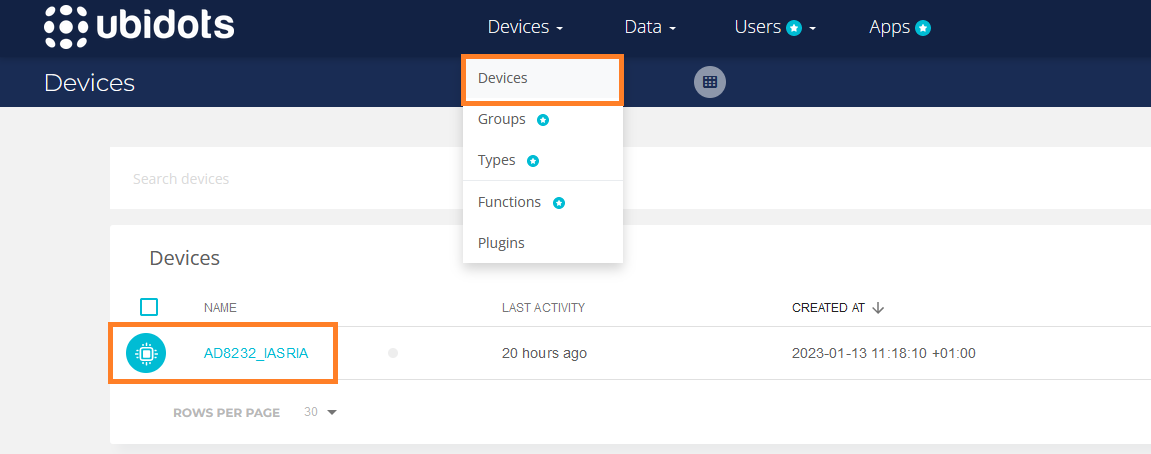
\includegraphics[width=\textwidth]{imgs/newdevice.png}
  \caption{Description du capteur AD8232 \label{newdevice}}
\end{figure}

La plateforme offre une large variante de composants comme la montre la figure \ref{devices}

\begin{figure}[H]
  \centering
  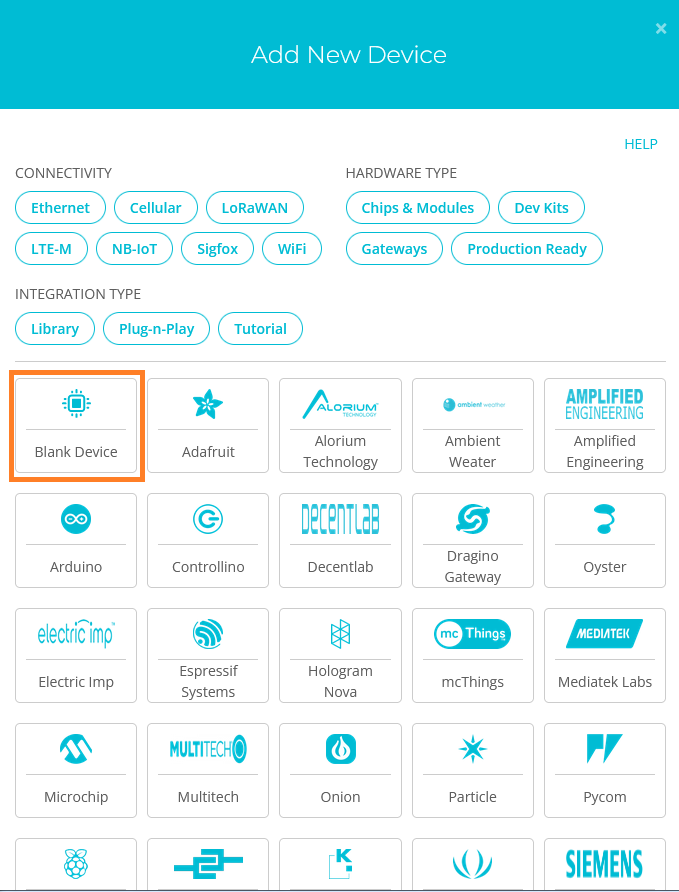
\includegraphics[scale=.4]{imgs/devices.png}
  \caption{Description du capteur AD8232 \label{devices}}
\end{figure}

Maintenant, il faut attribuer une variable à ce composant comme le montre la figure \ref{addnewdevice}

\begin{figure}[H]
  \centering
  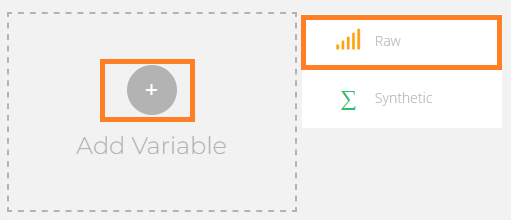
\includegraphics[scale=.4]{imgs/addnewdevice.png}
  \caption{Description du capteur AD8232 \label{addnewdevice}}
\end{figure}

Finalement, la variable \mintinline{c++}{ecg_val} est créé comme le montre la figure \ref{ecg_val}. Cette variable est utilisée par le programme afin de communiquer les données au capteur à la plateforme (voir l'appendix \ref{codesource}).

\begin{figure}[H]
  \centering
  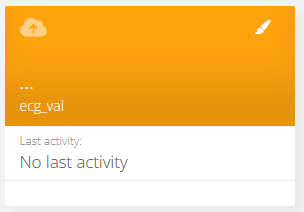
\includegraphics[scale=.4]{imgs/ecg_val.png}
  \caption{Description du capteur AD8232 \label{ecg_val}}
\end{figure}

D'un autre coté, il faut ajouter un nouveau dashboard pour visualiser les données, comme le montre la figure \ref{dashboard}

\begin{figure}[H]
  \centering
  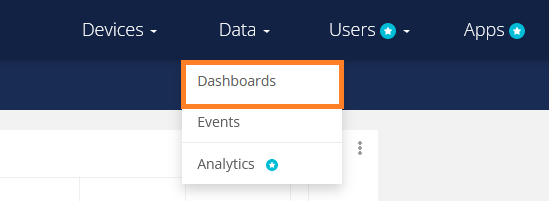
\includegraphics[scale=.4]{imgs/dashboard.png}
  \caption{Description du capteur AD8232 \label{dashboard}}
\end{figure}

Une grande variété de widgets est offerte afin de s'adapter aux différents besoins de l'utilisateur. Comme nous retraçons l'activité électirique cardiaque, nous voulons voir son évolution sous forme d'une courbe comme le montre la figure \ref{newwidget}

\begin{figure}[H]
  \centering
  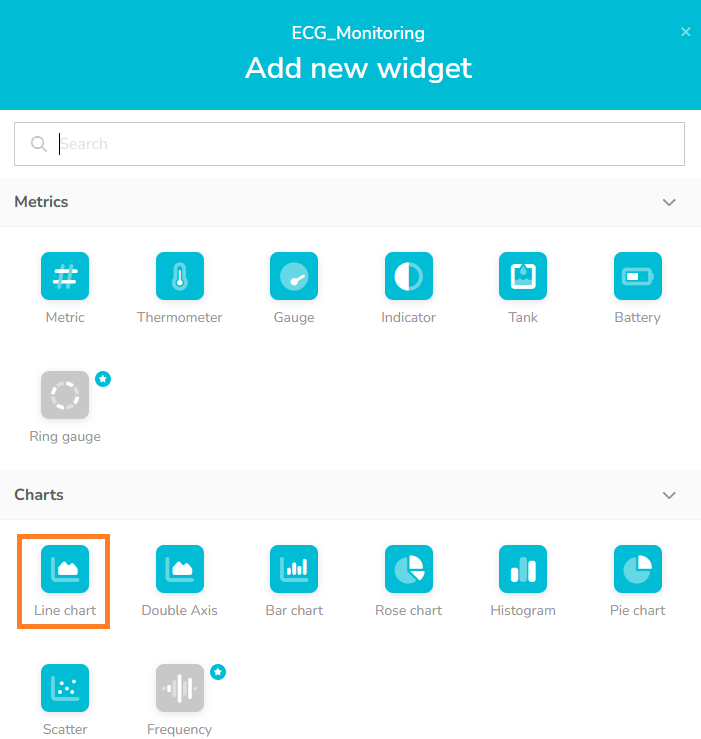
\includegraphics[scale=.4]{imgs/newwidget.png}
  \caption{Description du capteur AD8232 \label{newwidget}}
\end{figure}